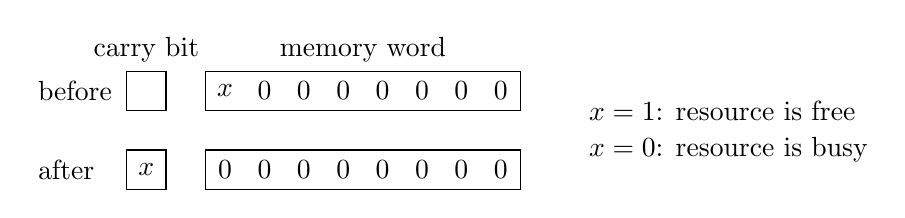
\begin{tikzpicture}[xscale=0.5]
\foreach \x/\t in {0/,2/x,3/0,4/0,5/0,6/0,7/0,8/0,9/0} {
  \node (X\x) at (\x,0) {$\t$};
}
\foreach \x/\t in {0/x,2/0,3/0,4/0,5/0,6/0,7/0,8/0,9/0} {
  \node (Y\x) at (\x,-1) {$\t$};
}
\draw (1.5,-0.25) rectangle (9.5,0.25);
\draw (1.5,-1.25) rectangle (9.5,-0.75);
\draw (-0.5,-0.25) rectangle (0.5,0.25);
\draw (-0.5,-1.25) rectangle (0.5,-0.75);
\draw (5.5,0.25) node[anchor=south] {memory word};
\draw (0,0.25) node[anchor=south] {carry bit};
\draw (-3,0) node[anchor=west] {before};
\draw (-3,-1) node[anchor=west] {after};
\draw (11,-0.25) node[anchor=west] {$x=1$: resource is free};
\draw (11,-0.75) node[anchor=west] {$x=0$: resource is busy};
\end{tikzpicture}